\documentclass[conference]{IEEEtran}
\usepackage{cite}
\usepackage{amsmath,amssymb,amsfonts}
\usepackage{algorithmic}
\usepackage{graphicx}
\usepackage{textcomp}
\usepackage{xcolor}
\usepackage{minted}
\def\BibTeX{{\rm B\kern-.05em{\sc i\kern-.025em b}\kern-.08em
    T\kern-.1667em\lower.7ex\hbox{E}\kern-.125emX}}
\begin{document}

\title{RustHDL and RHDL - two ongoing experiments in using Rust as a Hardware Description Language}

\author{\IEEEauthorblockN{Samit Basu}
  Fremont, California
  USA
  basu.samit@gmail.com
}

\maketitle

\begin{abstract}
  RustHDL and RHDL are two ongoing experiments in the use of the Rust programming language for the
  purposes of hardware description.  Both are open source projects that aim to bring the benefits
  of the Rust programming language to the task of firmware design, and focus on enabling the use
  of features such as strong typing, ease of design reuse, and rigorous safety and linting in
  the implementation of firmware.  RustHDL is the older of the two projects, has a fairly extensive
  library of IP cores for common hardware tasks, and has been fielded in commercial systems.
  RHDL is a next generation version of RustHDL that attempts to address some of its shortcomings.
  This paper attempts to describe both along with the rationale for the rewrite.
\end{abstract}

\begin{IEEEkeywords}
  Hardware description languages, Rust Programming Language, Field Programmable Gate Arrays,
  Design automation
\end{IEEEkeywords}


% Key ideas
% - Using a subset of RPL & RPL as a Host -> type checking, debugging, etc. for free
% - Interop with Verilog
% - High performance simulation & testing

\section{Introduction}
There are a number of new hardware description languages (HDL) that are being introduced that
attempt to remedy some of the shortcomings of the traditional Verilog or VHDL based workflow.
These HDLs tend to focus on newer features borrowed from the rapidly advancing fields of
software programming language design and compiler development.  Typically, these new HDLs
come with custom toolchains, new syntaxes and grammers, as well as new ways of thinking about
how hardware designs should best be expressed in text.

There is, however, an additional challenge that cannot be understated.  Hardware development
is typically quite difficult for those with traditional software engineering backgrounds.
The procedural, imperative mode of software development does not lend itself naturally to
the design of hardware systems.  Furthermore, true parallelism is quite difficult to manage in
most mainstream programming languages, and the techniques for sharing state across different
parts of a software program do not lend themselves to hardware designs and implementation.

The result of these difficulties lead to the development of two frameworks for describing
hardware using the Rust Programming Language.  The first of these two frameworks, called
RustHDL is older, and has substantial development effort along with commercial products
that have been shipped and are running using firmware written with it.  However, as more
people began to use RustHDL (and people with Rust background in particular), shortcomings
became evident in its design that lead to a rewrite that is known as RHDL.  Both of
these open source projects explore the use of the Rust programming language and its
suitability for the description of hardware designs.  Although the focus is on Field Programmable
Gate Arrays (FPGAs), the work is likely applicable to other fields of design as long as
the basic principles are preserved.

The key components of both frameworks are:
\begin{itemize}
\item The use of the type system to allow for description of complex data without
  a synthesis overhead, and independent of the underlying toolchains support for
  types.
\item The use of composition and simple structs to describe hierarchies of design
  with encapsulation and the hiding of internal details.
\item The use of Rust itself as the programming language.  No new grammar is required
  and all of the tooling that comes with the Rust programming language, including training,
  tooling, and infrastructure ``just work'' with both frameworks.  As a side effect,
  significant issues such as code sharing, documentation, and automated testing of hardware designs 
  are all handled by the Rust ecosystem.
\item The ability to integrate external IP cores and legacy designs (e.g., memory controllers,
  serializer/deserializers, PLLs, etc.) which cannot be described from first principles.
\item High performance simulation of hardware designs is built into the framework, so that
  testbenches and verification can be performed without the use of additional tools.
\end{itemize}

The organization of this paper is as follows.  Section~\ref{sec:related} describes related
works.  This is a particularly fruitful time for innovation in this space, and only a
sample of projects are discussed, primarily in their relationship to RustHDL and/or RHDL.
Section~\ref{sec:basics} describes the basics of how Rust is used as an HDL using the RustHDL
framework.  Section~\ref{sec:rhdl} describes how RHDL addresses the shortcomings discovered
during the development of RustHDL, with a particular focus on support for algebraic data types
and Rust syntax.  This section also touches briefly on the internals of the RHDL compiler and
how it cooperates with the Rust compiler.  Section~\ref{sec:roadmap} describes the roadmap for
the future of RHDL, and describes some of the limitations that could not be overcome.  Conclusions
and lessons learned are presented Section~\ref{sec:summary}.

\section{Background}

In considering the scope of background work, we will focus on the use of the Rust programming
language as primary in the consideration of Hardware Design Languages.  There are many modern
approaches to HDL in development (see [spade] and the references therein for a good overview).  
From a high level, however, programming languages can influence HDLs in one of two ways:

\begin{itemize}
  \item Through grammar similarity.  A number of HDLs use syntaxes that are inspired or similar to
  programming languages in order to make the transition from software to hardware design easier.
  For example, Chisel [chisel] uses a Scala-like syntax, and Spade [spade] uses a Rust-like syntax.
  The underlying implementation language is irrelevant (it happens to be Rust in the case of Spade).
  What is important is that the background experience and knowledge of the developer can be brought 
  to bear when understanding hardware descriptions if they use syntax and patterns from a broadly
  used programming language.
  \item As a host environment for the design.  In this case, a subset of the programming language (
    very similar in nature to a "synthesizable subset") is carved out of the broader programming language
    through some means, and then used to generate hardware designs within the context of the overall
    programming language.  An example here is MyHDL, which uses Python as the host language, and 
    designs are expressed in a subset of Python that is synthesizable into Verilog.
\end{itemize}

While there are several examples of HDLs that use Rust as the inspiration language, RustHDL and
RHDL fall into the second category, and the author could find no other examples like them.  In the 
first category, the most prominent examples are XLS [xls] and Spade [spade] and Veryl [veryl].  
In all three of these cases, the language is inspired by the syntax of Rust, and usually the type
system, but the actual tooling is separate from the Rust programming language and ecosystem.

RustHDL and RHDL are different in that \emph{hardware designs are expressed as valid Rust programs}.
This means that before a design can be synthesized, it must first pass the checks of the Rust
compiler.   It also means that much of the infrastructure of the Rust programming language can be reused
by hardware designers.  Things like package management, documentation, test management and IDE 
integration all come for free.

Finally, there is a rich history of using functional programming languages to describe HDL, and
with good reason.  RHDL in particular focuses on the functional aspects of Rust, and as a result 
provides some additional benefits to designers.  And both RustHDL and RHDL allow for high performance 
multithreaded simulation of the designs, all from within the same Rust ecosystem.

\section{RustHDL Basics}

RustHDL uses two aspects of the Rust programming language to describe hardware designs.  The first
is the use of traits.  An example is quite instructive, so here is an example of a simple strobe
circuit, written in RustHDL, and provided in the widget library that is published on crates.io.  Like 
every circuit desribed in RustHDL, it consists of three parts.  The first is the definition of the
circuit components, which includes input and output signals, as well as any internal components.
The use of Rust's \verb|pub| mechanism is used to hide internal details that should not be accessed
outside of the circuit.  The struct essentially describes the architecture of the circuit, including
input and output ports, types, and internal structure.

\begin{minted}[fontsize=\footnotesize]{rust}
use rust_hdl_core::prelude::*;
use crate::{dff::DFF, dff_setup};

/// A [Strobe] generates a periodic pulse train, 
/// with a single clock-cycle wide pulse
/// at the prescribed frequency.  The argument 
/// [N] of the generic [Strobe<N>] is used
/// to size the counter that stores the internal 
//  delay value.  
#[derive(Clone, Debug, LogicBlock)]
pub struct Strobe<const N: usize> {
    /// Set this to true to enable the pulse train.
    pub enable: Signal<In, Bit>,
    /// This is the strobing signal 
    /// it will fire for 1 clock cycle such that 
    /// the strobe frequency is generated.
    pub strobe: Signal<Out, Bit>,
    /// The clock that drives the [Strobe].  
    /// All signals are synchronous to this clock.
    pub clock: Signal<In, Clock>,
    threshold: Constant<Bits<N>>,
    counter: DFF<Bits<N>>,
}
\end{minted}

A couple of additional observations.  Signals have both a direction and a type.  The type of
signal can be any Rust type that implements the \verb|Synth| trait, and can include custom user
types and structs.  The \verb|derive| macro is used to generate the necessary boilerplate to make the 
\verb|Strobe| struct implement the \verb|Block| and \verb|Logic| traits.  The details of these implementations are
unimportant, and the user can simply use the \verb|Strobe| struct as if it were a normal Rust struct.  Also,
the D-type flip flop (DFF), which is critical to synchronous designs, is simply another circuit element that
is included in the internal structure of the \verb|Strobe| struct.  The RustHDL DFF is parameterized or 
generic over the type of data it holds, so in this case, it is holding an N-bit wide value.  The value of
\verb|N| is provided when the strobe is created.

The second part of the circuit encapsulates its behavior.  This is done by implementing the \verb|Logic| trait,
and requires only a single function, called \verb|update|:

\begin{minted}[fontsize=\footnotesize]{rust}
impl<const N: usize> Logic for Strobe<N> {
  #[hdl_gen]
  fn update(&mut self) {
    // Connect the counter clock to my clock
    dff_setup!(self, clock, counter);
    if self.enable.val() {
      self.counter.d.next = self.counter.q.val() + 1;
    }
    self.strobe.next = self.enable.val() & 
      (self.counter.q.val() == self.threshold.val());
    if self.strobe.val() {
      self.counter.d.next = 1.into();
    }
  }
}
\end{minted}

Here, the \verb|#[hdl_gen]| attribute is attached to the \verb|update| function to provide a way to convert the function
into Verilog.  The key thing to note, however, is that \emph{without this attribute, the function is still a valid Rust function}.
This means that the \verb|update| function can be tested, debugged, and run as a normal Rust function.  The \verb|#[hdl_gen]| adds
additional constraints to the code to ensure that it is synthesizable, but the Rust compiler still does the work of ensuring that the 
program input is correct.

The \verb|update| function follows a few rules that are laid out in the documentation.  In short:
\begin{itemize}
  \item Signals have two endpoints.  A \verb|.val()| endpoint that represents their current value, and a \verb|.next| endpoint that represents
    the value that the circuit is driving them to.
  \item Several Rust flow control primitives are allowed, including \verb|match, if| and a very limited \verb|for|.  
  \item The ideas of blocking and non-blocking assignments, which are confusing from a software perspective are removed.  
  \item Local variables are allowed, but they must be declared in the architecture of the circuit, like any other element.
  These signals have a type fo \verb|Local|, and are declared as \verb|my_sig: Signal<Local, T>|.
\end{itemize}

The last part of the circuit is the construction and initialization.  Here again, there is nothing special in RustHDL.  The 
constructor function is just a normal Rust function that populates the contents of the struct.  Because it can do anything
that a normal Rust function can do, arbitrary checks and computations (which are done prior to hardware synthesis) can be 
accomplished in the constructor.  For completeness, here is the constructor for the \verb|Strobe|, which includes some checks 
and takes frequencies as inputs (edited down for brevity):

\begin{minted}[fontsize=\footnotesize]{rust}
impl<const N: usize> Strobe<N> {
  pub fn new(frequency: u64, strobe_freq_hz: f64)
      -> Self {
    let clock_duration_femto = 
      freq_hz_to_period_femto(frequency as f64);
    let strobe_interval_femto = 
      freq_hz_to_period_femto(strobe_freq_hz);
    let interval = 
      strobe_interval_femto / clock_duration_femto;
    let threshold = interval.round() as u64;
    assert!((threshold as u128) < 
      (1_u128 << (N as u128)));
    assert!(threshold > 2);
    Self {
        enable: Signal::default(),
        strobe: Signal::default(),
        clock: Signal::default(),
        threshold: Constant::new(threshold.into()),
        counter: Default::default(),
    }
  }
}
\end{minted}

Note the presence of the \verb|assert!| statements, which ensure that the circuit parameters are valid for the given configuration, and
can spot issues before the circuit can even be constructed.  Unfortunately, Rust does not currently support much in the way of computation with generic parameters such as the 
size of the internal counter \verb|N| for the strobe.  As a result, checks are made at construction time to ensure that 
counter is wide enough to not roll over before the next strobe is generated.

\section{Simulation and Testing}

One powerful aspect of RustHDL and RHDL is the ease with which designs can be tested and simulated \emph{without} 
resorting to external tools.  For example, setting up a testbench for the \verb|Strobe| is quite simple.  Here is an example
for the \verb|Blinky| example from the documentation for RustHDL:

\begin{minted}[fontsize=\footnotesize]{rust}
fn main() {
  // v--- build a simple simulation using
  //  the simple_sim! macro for 1 clock, and
  //  only 1 testbench.
  let mut sim = simple_sim!(Blinky, clock, 
      CLOCK_SPEED_HZ, ep, 
    {
      // v--- The testbench code goes here.
      let mut x = ep.init()?;
      wait_clock_cycles!(ep, clock, 
        x, 4*CLOCK_SPEED_HZ);
      ep.done(x)
    }
  );
  // v--- construct the circuit
  let uut = Blinky::default();
  // v--- run the simulation, with the 
  // output traced to a .vcd file
  sim.run_to_file(Box::new(uut), 
    5*sim_time::ONE_SEC, "blinky.vcd")
    .unwrap();
}
\end{minted}

In this simple example, the simulation simply creates a trace file that can then be inspected visually.  While this 
is sufficient for simple circuits, more complex designs will require sophisticated testbenches.  Fortunately, RustHDL
allows the engineer to write those testbenches using the full power of Rust.  A more complex example is here (again, edited for
brevity, with the key parts left in place):

\begin{minted}[fontsize=\footnotesize]{rust}
  #[test]
fn test_hls_sdram_fifo_works() {
  let mut uut = HLSSDRAMFIFOTest::default();
  let mut sim = Simulation::new();
  // v-- generate random data using Rust
  let data = (0..256)
      .map(|_| rand::thread_rng().gen::<u16>())
      .collect::<Vec<_>>();
  let data2 = data.clone();
  // v-- generate the clock
  sim.add_clock(4000, |x: &mut Box<_>| {
      x.clock.next = !x.clock.val()
  });
  // v-- this testbench feed data to the fifo
  sim.add_testbench(move |mut sim: Sim<_>| {
      let mut x = sim.init()?;
      wait_clock_cycles!(sim, clock, x, 20);
      hls_fifo_write_lazy!(sim, clock, x, 
        fifo.bus_write, &data);
      sim.done(x)
  });
  // v-- this testbench drain data from the fifo
  //    and panic if it doesn't match the input
  sim.add_testbench(move |mut sim: Sim<_>| {
      let mut x = sim.init()?;
      wait_clock_cycles!(sim, clock, x, 20);
      hls_fifo_read_lazy!(sim, clock, x, 
        fifo.bus_read, &data2);
      sim.done(x)
  });
  // v-- both testbenches are run simultaneously
  sim.run_to_file(Box::new(uut), 200_000_000, 
      &vcd_path!("hls_sdram_fifo.vcd")).unwrap();
}
\end{minted}

This test harness sets up a SDRAM-backed FIFO (which is a fairly complex circuit) and then writes and reads a 
series of random values to the FIFO and reads them back \emph{simultaneously}.  This particular testbench includes
a full simulation of the underlying SDRAM itself, which is also modelled in RustHDL.  The resulting trace file is
quite complicated, but the testbench includes an assertion, and will panic if at any time the FIFO errors out.  The 
FIFO read and write macros include random delays that ensure that different edge conditions are likely to be tested 
during the run.  Again, this is difficult in a traditional HDL, but quite trivial in RustHDL.

\begin{figure*}[htbp]
  \centerline{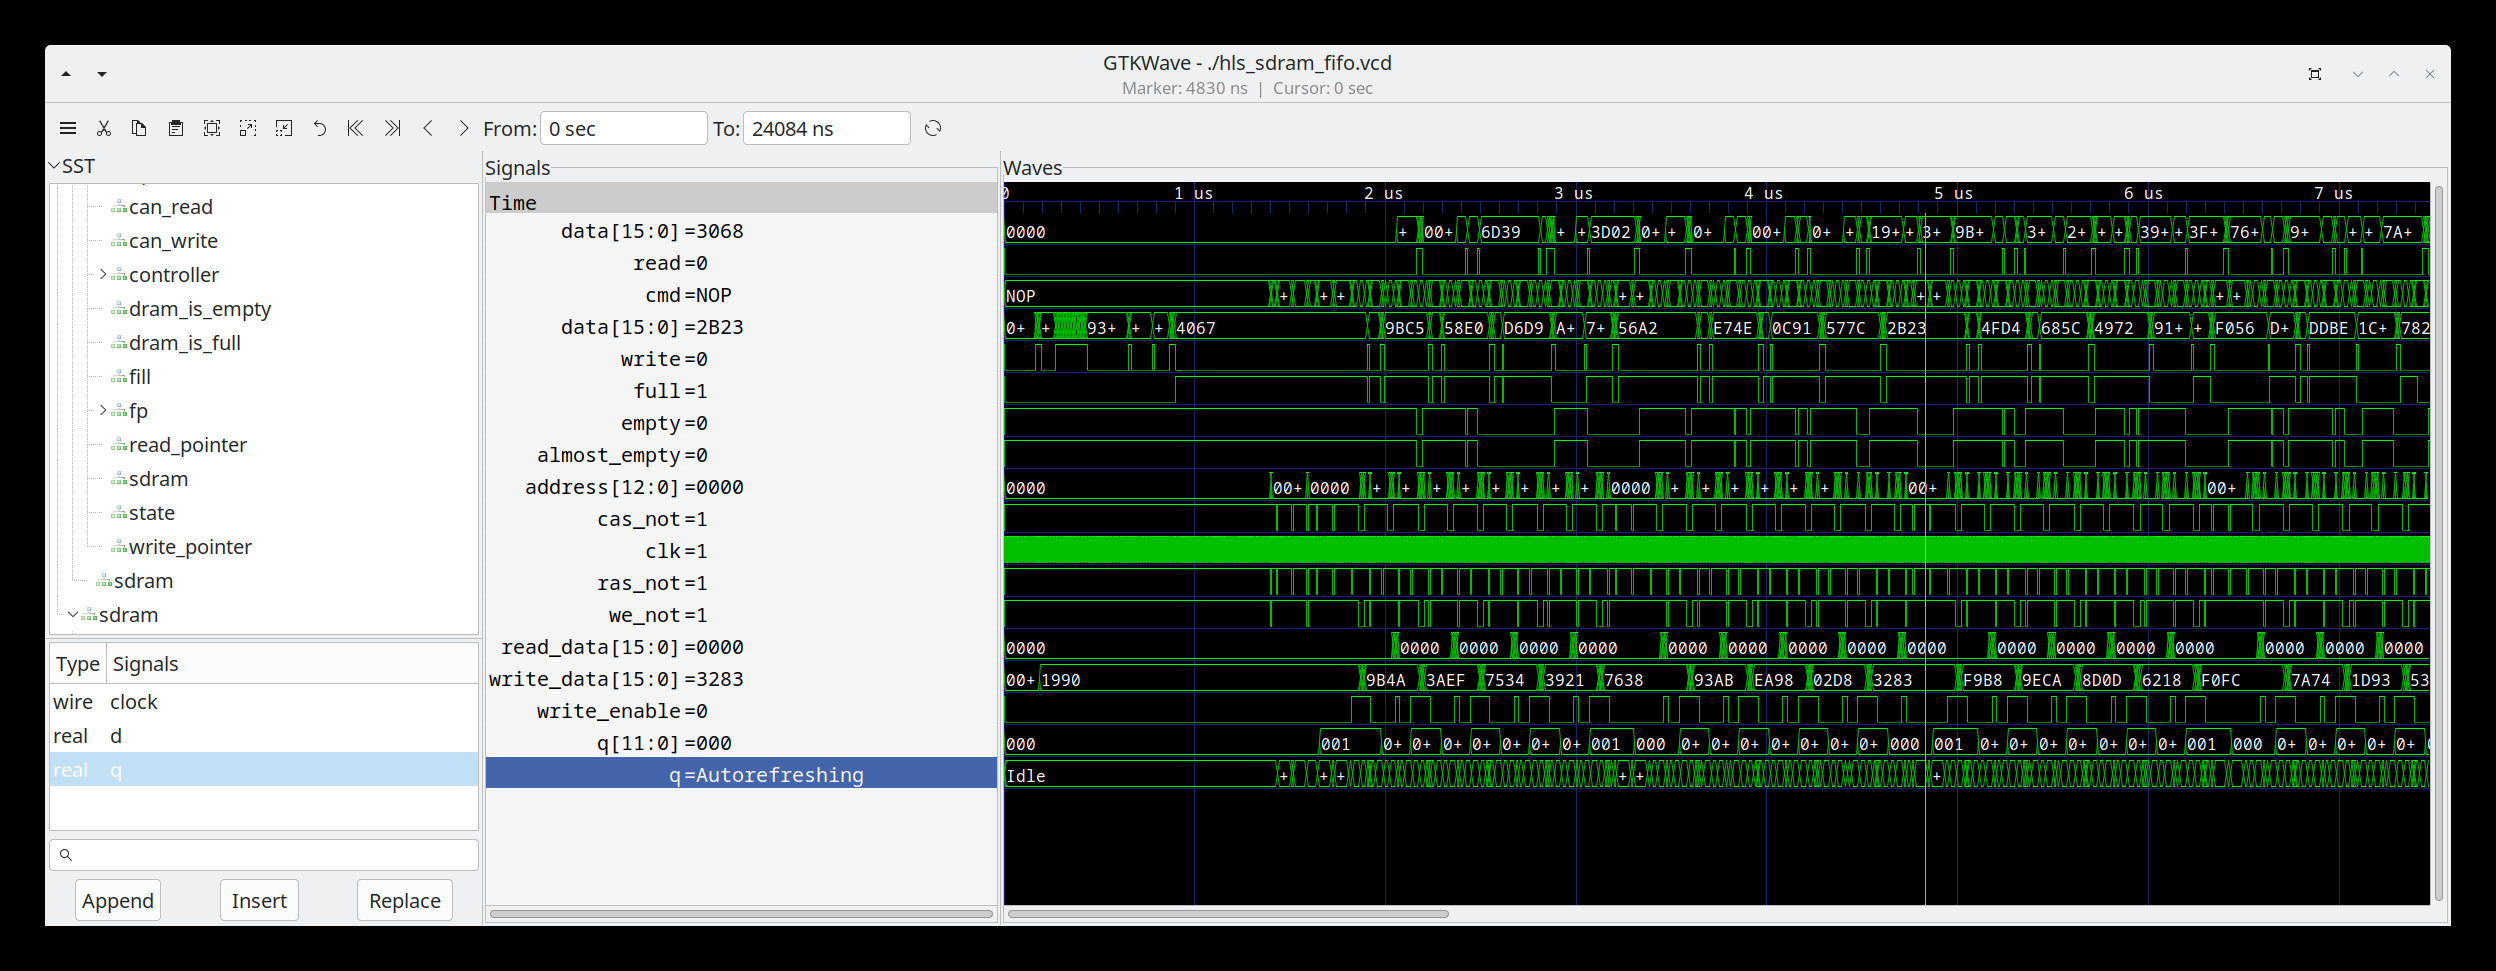
\includegraphics[width=18cm]{hls_sdram_fifo.png}}
  \caption{Sample simulation trace for the \textrm{HLSSDRAMFIFOTest} testbench}
  \label{fig}
\end{figure*}
  
Finally, executing the full test suite of RustHDL is as simple as executing the standard \verb|cargo test| command from a 
checkout of the code.  The only caveat is that several of the tests require physical FPGAs to be connected to the host
machine to operate, and require vendor specific software (synthesis tools, communication libs, etc).  However, most 
of the cores are tested using software only frameworks.

\section{Synthesis}

Obviously, to get a RustHDL design onto an FPGA, it must be synthesized.  The process is simple.  Given a struct that
implements the required \verb|Logic| trait, the equivalent Verilog description of the circuit can be generated with a simple
command:

\begin{minted}[fontsize=\footnotesize]{rust}
  fn main() {
    // v--- Create the circuit
    let mut uut = Blinky::default();
    // v--- Internal wiring
    uut.connect_all(); 
    let vlog = generate_verilog(&uut);
    // v--- Write the verilog to the console
    println!("{vlog}"); 
}
\end{minted}

The resulting Verilog can then be synthesized using standard tools.  In the course of development the author used 
open source tools when possible (including yosys and nextpnr), but also used vendor tools (ISE, Vivado and Diamond)
when necessary.  Designs that used a fair amount of a moderate sized FPGA and included state machines, data transfer 
mechanisms, SPI controllers, SDRAM controllers, and other components were all built, simulated in Rust, and then
synthesized and tested with physical devices.  While there were definitely issues encountered in which the synthesized 
results did not match the expectation, in most cases those issues were a result of bugs in the synthesis toolchain, and not
in the generated output.

As a further advantage of the use of Rust for the design language, a number of side "effects" can also be handled 
efficiently as part of the synthesis process.  The main issue that one typically encounters is the need to enumerate
and attach constraints to different parts of the design.  These constraints (for FPGAs), indicate things like 
voltage levels, if drivers are paired up differentially or are tristated, etc.  Timing constraints are also needed,
especially when signals come from off-chip or need to meet certain setup and hold constraints.  

For the most part, constraints are highly vendor specific, and thus there is not much that can be done to provide
a universal framework for specifying them.  However RustHDL at least provides a degree of organization to the constraints.
In fact, RustHDL proposes the use of a "Board Support Package" (as is typically used in the embedded world) to provide 
both the toolchain configuration and constraints needed for the FPGA of interest.  

As a trivial example of this flexibility, consider the following code snippet from the BSP for the Alchitry Cu board:

\begin{minted}[fontsize=\footnotesize]{rust}
pub fn leds() -> Signal<Out, Bits<8>> {
  let mut x = Signal::<Out, _>::default();
  for (ndx, uname) in ["J11", "K11", "K12", ...]
      .iter()
      .enumerate()
  {
      x.add_location(ndx, uname);
  }
  x
}
\end{minted}

This simple function provides a signal with 8 bits, each of which is pre-constrained to indicate which pin on the 
FPGA is connected to the corresponding LED.  That information can now be used in any design that needs an LED 
indicator with a fair degree of device independence.  Similarly, synthesizing a design for the Alchitry Cu board 
is handled by a function

\begin{minted}[fontsize=\footnotesize]{rust}
pub fn generate_bitstream<U: Block>
    (mut uut: U, prefix: &str) {}
\end{minted}

This function takes any struct that implements a design (with the constraints already attached to the relevant
signals), and a directory location to place the intermediate files.  It then generates the Verilog description of
the design, and invokes \verb|yosys| and \verb|nextpnr| followed by \verb|icepack| to generate a bitfile for the ICE40 FPGA on the
AlchitryCu board.  Equivalent functions provide support for Xiling Spartan-6 and Artix-7 FPGAs, as well as Lattice ECP5 parts.

\section{Interoperability}

There are three key aspects to interoperability in RustHDL:

\begin{enumerate}
  \item The separation of interfaces from implementations.
  \item The ability to use existing IP cores and designs in a RustHDL design.
  \item The ability to use RustHDL designs in existing Verilog or VHDL designs.
\end{enumerate}

For the first item, consider the following example from the Xilinx Spartan-6 BSP:

\begin{minted}[fontsize=\footnotesize]{rust}
#[derive(Clone, LogicInterface, Default)]
pub struct MCBInterface1GDDR2 {
    data_bus: Signal<InOut, Bits<16>>,
    address: Signal<Out, Bits<13>>,
    bank_select: Signal<Out, Bits<3>>,
    row_address_strobe_not: Signal<Out, Bit>,
    column_address_strobe_not: Signal<Out, Bit>,
    // snip
    chip_select_neg: Signal<Out, Bit>,
}
\end{minted}

This struct, annotated with \verb|LogicInterface| instead of \verb|LogicBlock| represents a set of signals that are used
to connect to a DRAM controller.  The \verb|LogicInterface| trait is similar to the \verb|Logic| trait, but does not include
an \verb|update| function.  Interfaces allow entire groups of signals to be described with a single element of the
top level struct.  For example, the \verb|MCBInterface1GDDR2| is included in the memory interface generator (MIG) generated 
by the Xilinx tools, which itself is wrapped into an RustHDL struct.

\begin{minted}[fontsize=\footnotesize]{rust}
#[derive(LogicBlock)]
pub struct MemoryInterfaceGenerator {
    // Raw clock from the system - 
    pub raw_sys_clk: Signal<In, Clock>,
    // Reset - must be handled externally
    pub reset: Signal<In, Bit>,
    // Calibration complete
    pub calib_done: Signal<Out, Bit>,
    // ..snip..
    // P0 read port
    pub p0_rd: ReadPort,
    // MCB interface
    pub mcb: MCBInterface1GDDR2,
    // FIFO for the commands
    cmd_fifo: AsynchronousFIFO<MIGCommand, 2, 3, 1>,
    // ..snip..
}
\end{minted}  

Even with the very basic description of RustHDL presented so far, this description of the memory interface generator (MIG) (which is a
fairly complicated piece of hardware) is quite simple.   Through some wrapper code, this interface is connected to a black Box
IP instantiation that is ultimately turned by the synthesis tools into a functioning design.  For simulation purposes, a version 
of the MIG that is implemented in fabric using a BRAM is used, and the interface is connected to that instead.  The result is that
a design can be generated that can be run on any FPGA (even one with out the necessary hardware) for verification and testing.


Finally, one of the original use cases for RustHDL was to generate IP cores that could be utilized by engineers using traditional 
techniques and HDL languages.  To that end the output of RustHDL was meant to be human readable Verilog.  This is an important 
feature, since things like timing analysis and other tools will typically report issues using the Verilog as a reference.  If the
Verilog is unstructured and difficult to read, then the ability to map e.g., a critical timing path back to the original source 
code can be quite difficult.  RustHDL attempts to generate Verilog that is as close to the original source as possible, with 
various renaming and unrolling transformations to account for features missing in Verilog or identifiers that are illegal in 
one language or the other.  As an example of this preservation of syntax, the following is an example of a generated top level
Verilog for a simple LED blinker:

\begin{minted}[fontsize=\footnotesize]{verilog}
module top(clock,leds);
  
  // Module arguments
  input wire  clock;
  output reg  [7:0] leds;
  
  // Stub signals
  reg  pulser$clock;
  reg  pulser$enable;
  wire  pulser$pulse;
  
  // Sub module instances
  top$pulser pulser(
      .clock(pulser$clock),
      .enable(pulser$enable),
      .pulse(pulser$pulse)
  );
  
  // Update code
  always @(*) begin
      pulser$enable = 1'b1;
      pulser$clock = clock;
      leds = 32'h0;
      if (pulser$pulse) begin
          leds = 32'haa;
      end
  end  
endmodule // top
\end{minted}

The equivalent RustHDL code is:

\begin{minted}[fontsize=\footnotesize]{rust}
#[derive(LogicBlock)]
pub struct AlchitryCuPulser {
    pulser: Pulser,
    clock: Signal<In, Clock>,
    leds: Signal<Out, Bits<8>>,
}

impl Logic for AlchitryCuPulser {
    #[hdl_gen]
    fn update(&mut self) {
        self.pulser.enable.next = true;
        clock!(self, clock, pulser);
        self.leds.next = 0x00.into();
        if self.pulser.pulse.val() {
            self.leds.next = 0xAA.into();
        }
    }
}
\end{minted}

The code is essentially 1-to-1 transformed, which is both a benefit and a drawback of RustHDL.  This and other issues 
are discussed in the next section.

\section{Lessons Learned and the Path to RHDL}

RustHDL has been used to develop commercial grade firmware and is deployed in commercial products.  It has also seen 
some level of adoption by the open source community, with third party crates published on \verb|crates.io| that add board
support packages to RustHDL for different FPGAs, or augment the capabilities of the framework.  However, based on
feedback from users getting started with the framework, the following items became clear:

\begin{itemize}
  \item Engineers coming to a Rust-based HDL environment are likely to be familiar with the Rust programming language,
  and have grown accustomed to patterns and language features that are not supported by RustHDL.  For example, the 
  use of \verb|match| \emph{expressions}, and the use of complex types with their need to employ pattern matching to destructure 
  them are all idiomatic in Rust, but not supported by RustHDL.  This 
  lack of support stems from the close connection to Verilog of the generated code.
  \item Many idiomatic Rust patterns require some kind of support for Algebraic (Sum) Data Types (ADTs).  While RustHDL
  supports simple C-style enums, that is not sufficient to express many of the patterns common in Rust, including the 
  \verb|Result| and \verb|Option| patterns.
  \item The need to declare all local variables and their types up front is cumbersome.  Being able to freely rebind
  names and assign them is also critical to several standard Rust patterns (like shadowing).  This is also not
  possible in RustHDL.
  \item Functions cannot be chained together, i.e. composition of functions is not possible.
  \item Testing is somewhat clunky.  Testbenches are written in Rust, but require an understanding of the underlying
  event-based simulator that is used.  This makes testbenches difficult to write, and makes it difficult to use those
  testbenches in other environments (e.g., Verilog).
  \item No analysis is provided.  While RustHDL should be able to identify, e.g., timing issues, potential sources of
  metastability, or long paths in design, it does not.  This is primarily a result of the lack of a higher order model
  of the design being constructed within RustHDL, which looks mostly at one module at a time.
  \item Backends for multiple HDLs were requested, including FIRTL, VHDL and others.  Some of those backends support
  rich type information to be carried on signals, and so would benefit from propogating that typed information through
  to the HDL instead of simply generating bit vectors.
\end{itemize}

After taking all of these considerations into account, a new framework, named RHDL was planned that addressed these issues.  The 
core differences between RustHDL and RHDL are:

\begin{itemize}
  \item Full support for Rust data types, including ADTs, tuples, etc.
  \item Full support of Rust syntax inside functions (with the exception of pointers), which includes 
  match and if \emph{expressions}, early returns, etc.
  \item Full support for function composition.
  \item Support for local variables/rebindings, as well as pattern matching in \verb|match| expressions.
  \item The use of a function iterator-style description of testbenches in which testbenches are written in 
  straight Rust, and consumed by the simulator (so that the details of how the circuit is simulated can be ignored).
  \item Support for thorough analysis of the design, including identification of potential timing issues, as well as
  metastability detection, and clock domain crossings.
  \item Support for multiple backend languages is possible, even for those that want type information.
\end{itemize}

These items required a signficantly broader scope and far more effort on the compiler side of the framework.  In particular,
the first four items required the development of a full compiler that works in conjuntion with \verb|rustc| to perform
type inference, as well as type checking, lowering of Rust expressions to an intermediate representation (which is a sort of
RTL-SSA assembly code), optimization passes, analysis passes, and finally, generation of the input to the synthesis tools.

This effort carried with it its own set of challenges, which this paper cannot describe or address.  Suffice to say, the RHDL
project is still in an early development phase.  While designs have been synthesized, it is still in the process of being
fleshed out.  A few pieces are of interest, though, so we describe them here.

\subsection{The Digital Trait}
RHDL introduces a \verb|Digital| trait, which is used to convert arbitrary Rust structs into bit vectors.  Here is an example from
the early RHDL work:

\begin{minted}[fontsize=\footnotesize]{rust}
  #[derive(Copy, Clone, PartialEq, Debug, Digital, Default)]
  #[rhdl(discriminant_width = 4)]
  enum Test {
      #[default]
      A,
      B(b2, b3),
      C {
          a: b8,
          b: b8,
      },
  }
\end{minted}

In this case \verb|b8| is an 8-bit unsigned value (there is also \verb|s8| for a signed 8 bit value).  The \verb|Digital| trait can be
auto derived on structs and enums, and is automatically supplied for arrays and tuples.  This very powerful trait allows 
complex data structures to be built and deconstructed safely with the compiler ensuring that bit accesses are always correct.
In this case, the discriminant width is specified at 4 bits (instead of the 2 bits it would naturally require).  The position 
of the discriminant can also be controlled with MSB and LSB positioning. 

\subsection{The \textrm{kernel} Attribute}
The \verb|kernel| attribute is used to mark functions that are to be synthesized.  While there are still limits on what 
functions can be processed, the limits are fairly broad (essentially, the inputs and outputs must be \verb|Digital| types). 
The compiler then deconstructs the kernel function and builds an intermediate form of it.  This is where support for
Rust constructs like early returns, match expressions, etc. are handled.   At this point, type inference is also needed, 
for intermediate local variables and pattern matching.  

This small snippet of RHDL demonstrates some of those principles in action:
\begin{minted}[fontsize=\footnotesize]{rust}
#[kernel]
pub fn blinker_update(params: Blinker, 
                        state: BlinkerState) -> 
                        (BlinkerState, b4) {
    // v- tuple destructuring, function chaining
    let (q_pulser, pulser_output) = 
        pulser_update(params.pulser, 
                      state.pulser, 
                      true);
    // v- if expression, type inference
    let blinker_output = if pulser_output {
        b4(0b1111)
    } else {
        b4(0b0000)
    };
    // v- tuple construction
    (
      BlinkerState { pulser: q_pulser }, 
      blinker_output
    )
}
\end{minted}
This function looks completely different than RustHDL, where an impure function with a \verb|mut self| argument
is replaced with a pure function with \verb|Digital| inputs.  The stages of the RHDL compilation are illustrated in 
Figure~\ref{fig:rhdl_compiler}.  In the current version, the output of the compiler is straight Verilog, but bears
little resemblance to the original source code.  As a result the need to perform timing analysis and other analysis
steps at the Rust level becomes more important.  RHDL also introduces an intermediate form named \verb|RHIF| which 
serves as a strongly typed RTL-assembly representation of the logic that obeys SSA rules.  As we will see in the
next subsection, this intermediate representation is critical for testing and code generation.

\subsection{Functional Testing and the Virtual Machine}
With the move to pure functions, testing becomes significantly simpler.  Indeed, RHDL allows an engineer to 
trivially test a kernel function at three levels:

\begin{enumerate}
  \item At the Rust level, where the logic of the function is being tested.
  \item At the RHIF level via a virtual machine, which tests the lowering of the Rust function to the lower 
  level hardware-synthesizable primitives.
  \item At the verilog level via an autogenerated testbench which includes the correct outputs as generated 
  by \verb|rustc|.
\end{enumerate}

The idea is to bootstrap off of the Rust compiler (which is highly unlikely to generate incorrect code), and progressively
test each additional level in the compilation process.  Because the functions are pure, they can, in principle, be
exhaustively tested if the inputs are small enough.  The process of doing this consists of a single function call (edited for brevity):

\begin{minted}[fontsize=\footnotesize]{rust}
#[test]
fn test_simple_if_expression() {
    #[kernel]
    fn foo(a: b8, b: b8) -> b8 {
        if a > b {
            a + 1
        } else {
            b + 2
        }
    }
    test_kernel_vm_and_verilog
       (foo, tuple_pair_b8()).unwrap();
}  
\end{minted}

In this example, the \verb|foo| function is tested at two of the three levels.  It is assumed that the 
Rust implementation and the output generated by \verb|rustc| are correct and as intended (this can be tested
with standard test infrastructure used for any normal Rust code).  Then the \verb|foo| function is compiled into RHIF, and
the resulting code is simulated using a virtual machine implementation.  The \verb|tuple_pair_b8| function simply returns an
iterator that yields all possible pairs of 8-bit values.  Finally, the verilog version of the function is 
generated, along with a testbench that iterates over all of the possible inputs and compares the result to 
the reference value from \verb|rustc|.  In this way, the engineer can have a high degree of confidence that if the Rust 
code is correct that the generated HDL will also be correct.  In the current RHDL implementation, that Verilog testbench
is executed using Icarus Verilog, but any other Verilog simulator could be used.  It is a powerful way to test 
the compiler and to ensure that the generated code is correct.


\section*{Acknowledgment}

The preferred spelling of the word ``acknowledgment'' in America is without 
an ``e'' after the ``g''. Avoid the stilted expression ``one of us (R. B. 
G.) thanks $\ldots$''. Instead, try ``R. B. G. thanks$\ldots$''. Put sponsor 
acknowledgments in the unnumbered footnote on the first page.

\section*{References}

Please number citations consecutively within brackets \cite{b1}. The 
sentence punctuation follows the bracket \cite{b2}. Refer simply to the reference 
number, as in \cite{b3}---do not use ``Ref. \cite{b3}'' or ``reference \cite{b3}'' except at 
the beginning of a sentence: ``Reference \cite{b3} was the first $\ldots$''

Number footnotes separately in superscripts. Place the actual footnote at 
the bottom of the column in which it was cited. Do not put footnotes in the 
abstract or reference list. Use letters for table footnotes.

Unless there are six authors or more give all authors' names; do not use 
``et al.''. Papers that have not been published, even if they have been 
submitted for publication, should be cited as ``unpublished'' \cite{b4}. Papers 
that have been accepted for publication should be cited as ``in press'' \cite{b5}. 
Capitalize only the first word in a paper title, except for proper nouns and 
element symbols.

For papers published in translation journals, please give the English 
citation first, followed by the original foreign-language citation \cite{b6}.

\begin{thebibliography}{00}
\bibitem{b1} G. Eason, B. Noble, and I. N. Sneddon, ``On certain integrals of Lipschitz-Hankel type involving products of Bessel functions,'' Phil. Trans. Roy. Soc. London, vol. A247, pp. 529--551, April 1955.
\bibitem{b2} J. Clerk Maxwell, A Treatise on Electricity and Magnetism, 3rd ed., vol. 2. Oxford: Clarendon, 1892, pp.68--73.
\bibitem{b3} I. S. Jacobs and C. P. Bean, ``Fine particles, thin films and exchange anisotropy,'' in Magnetism, vol. III, G. T. Rado and H. Suhl, Eds. New York: Academic, 1963, pp. 271--350.
\bibitem{b4} K. Elissa, ``Title of paper if known,'' unpublished.
\bibitem{b5} R. Nicole, ``Title of paper with only first word capitalized,'' J. Name Stand. Abbrev., in press.
\bibitem{b6} Y. Yorozu, M. Hirano, K. Oka, and Y. Tagawa, ``Electron spectroscopy studies on magneto-optical media and plastic substrate interface,'' IEEE Transl. J. Magn. Japan, vol. 2, pp. 740--741, August 1987 [Digests 9th Annual Conf. Magnetics Japan, p. 301, 1982].
\bibitem{b7} M. Young, The Technical Writer's Handbook. Mill Valley, CA: University Science, 1989.
\end{thebibliography}
\vspace{12pt}
\color{red}
IEEE conference templates contain guidance text for composing and formatting conference papers. Please ensure that all template text is removed from your conference paper prior to submission to the conference. Failure to remove the template text from your paper may result in your paper not being published.

\end{document}
